%%%%%%%%%%%%%%%%%%%%%%%%%%%%%%%%%%%%%%%%%
% University Assignment Title Page 
% LaTeX Template
% Version 1.0 (27/12/12)
%
% This template has been downloaded from:
% http://www.LaTeXTemplates.com
%
% Original author:
% WikiBooks (http://en.wikibooks.org/wiki/LaTeX/Title_Creation)
%
% License:
% CC BY-NC-SA 3.0 (http://creativecommons.org/licenses/by-nc-sa/3.0/)
% 
% Instructions for using this template:
% This title page is capable of being compiled as is. This is not useful for 
% including it in another document. To do this, you have two options: 
%
% 1) Copy/paste everything between \begin{document} and \end{document} 
% starting at \begin{titlepage} and paste this into another LaTeX file where you 
% want your title page.
% OR
% 2) Remove everything outside the \begin{titlepage} and \end{titlepage} and 
% move this file to the same directory as the LaTeX file you wish to add it to. 
% Then add \input{./title_page_1.tex} to your LaTeX file where you want your
% title page.
%
%%%%%%%%%%%%%%%%%%%%%%%%%%%%%%%%%%%%%%%%%

%----------------------------------------------------------------------------------------
%	PACKAGES AND OTHER DOCUMENT CONFIGURATIONS
%----------------------------------------------------------------------------------------

\documentclass[12pt]{article}
\usepackage[catalan]{babel}
\usepackage[utf8]{inputenc}
\usepackage{float}
\usepackage{graphicx}
\usepackage{wrapfig}
\usepackage{lscape}
\usepackage{rotating}
\usepackage{epstopdf}
\usepackage{makeidx}

\makeindex
\begin{document}

\begin{titlepage}

\newcommand{\HRule}{\rule{\linewidth}{0.5mm}} % Defines a new command for the horizontal lines, change thickness here

\center % Center everything on the page
 
%----------------------------------------------------------------------------------------
%	HEADING SECTIONS
%----------------------------------------------------------------------------------------

\textsc{\LARGE Universitat de Barcelona}\\[1.5cm] % Name of your university/college
\textsc{\Large Client-Servidor}\\[0.5cm] % Major heading such as course name
\textsc{\large Enfonsar la flota}\\[0.5cm] % Minor heading such as course title

%----------------------------------------------------------------------------------------
%	TITLE SECTION
%----------------------------------------------------------------------------------------

\HRule \\[0.4cm]
{ \huge \bfseries Pràctica 1}\\[0.4cm] % Title of your document
\HRule \\[1.5cm]
 
%----------------------------------------------------------------------------------------
%	AUTHOR SECTION
%----------------------------------------------------------------------------------------



% If you don't want a supervisor, uncomment the two lines below and remove the section above
\Large \emph{Author:}\\
Christian José \textsc{Soler}\\
Nicolás Martín \textsc{Forteza Ocaña}\\[3cm] % Your name

%----------------------------------------------------------------------------------------
%	DATE SECTION
%----------------------------------------------------------------------------------------

{\large \today}\\[3cm] % Date, change the \today to a set date if you want to be precise

%----------------------------------------------------------------------------------------
%	LOGO SECTION
%----------------------------------------------------------------------------------------

%\includegraphics{Logo}\\[1cm] % Include a department/university logo - this will require the graphicx package
 
%----------------------------------------------------------------------------------------

\vfill % Fill the rest of the page with whitespace

\end{titlepage}
\addcontentsline{toc}{section}{Índice alfabético}
\printindex
\section*{Introducció}
En aquesta pràctica se'ns demana implementar el joc d'Enfonsar la flota perquè juguin diferents Clients contra un mateix servidor.

L'objectiu del joc és endevinar la situació dels vaixells de l'enemic i enfonsar-los indicant les coordenades. Tot això entre un client i servidor que implementi el protocol especificat a l'enunciat.

L'objectiu d'implementar aquest programa és aprendre a utilitzar els mecanismes de programació Client/Servidor en Java. En concret aprendre a utilitzar l'API Socket de Java.net i a fer servidors multi-petició.

El Client haurà de tenir un mode manual i un mode automàtic per a jugar una única partida a l'hora, en canvi, el Server solament tindrà mode automàtic i podrà jugar diverses partides a l'hora gestionades en un cas per Threads i en un altre per un Selector.
Tot això s'haurà de fer fent un bon ús de la programació Orientada a Objectes en Java.

\newpage
\section*{Plantejament}

\newpage
\section*{Annex}
\begin{sidewaysfigure}[ht]
    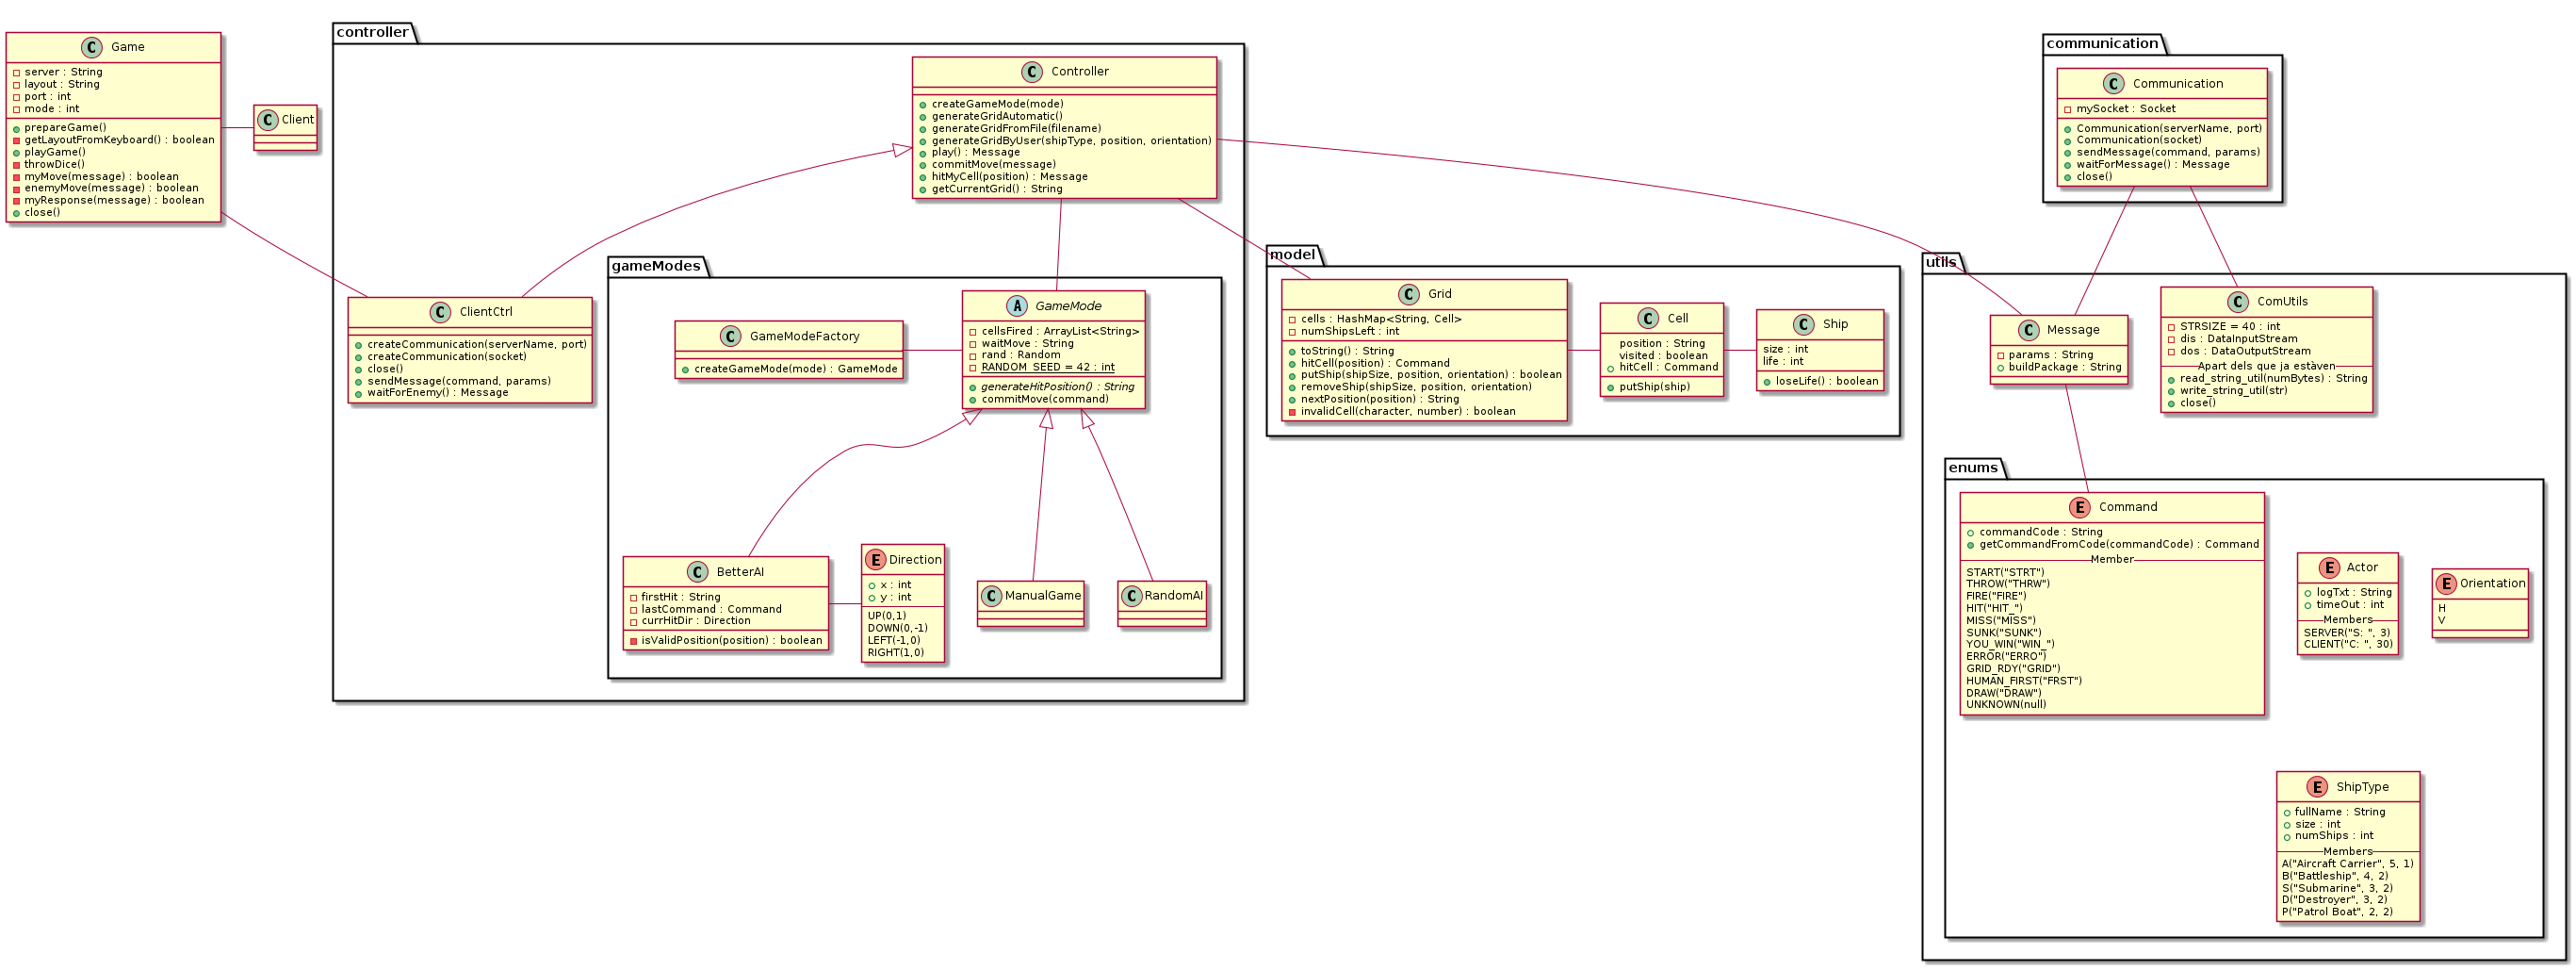
\includegraphics[width=\textwidth,height=\textheight,keepaspectratio]{../diagrams/class-diagrams/clientClasses.png}
    \caption{Client Diagram}
    \label{fig:PropProf}
\end{sidewaysfigure}
\begin{sidewaysfigure}[ht]
    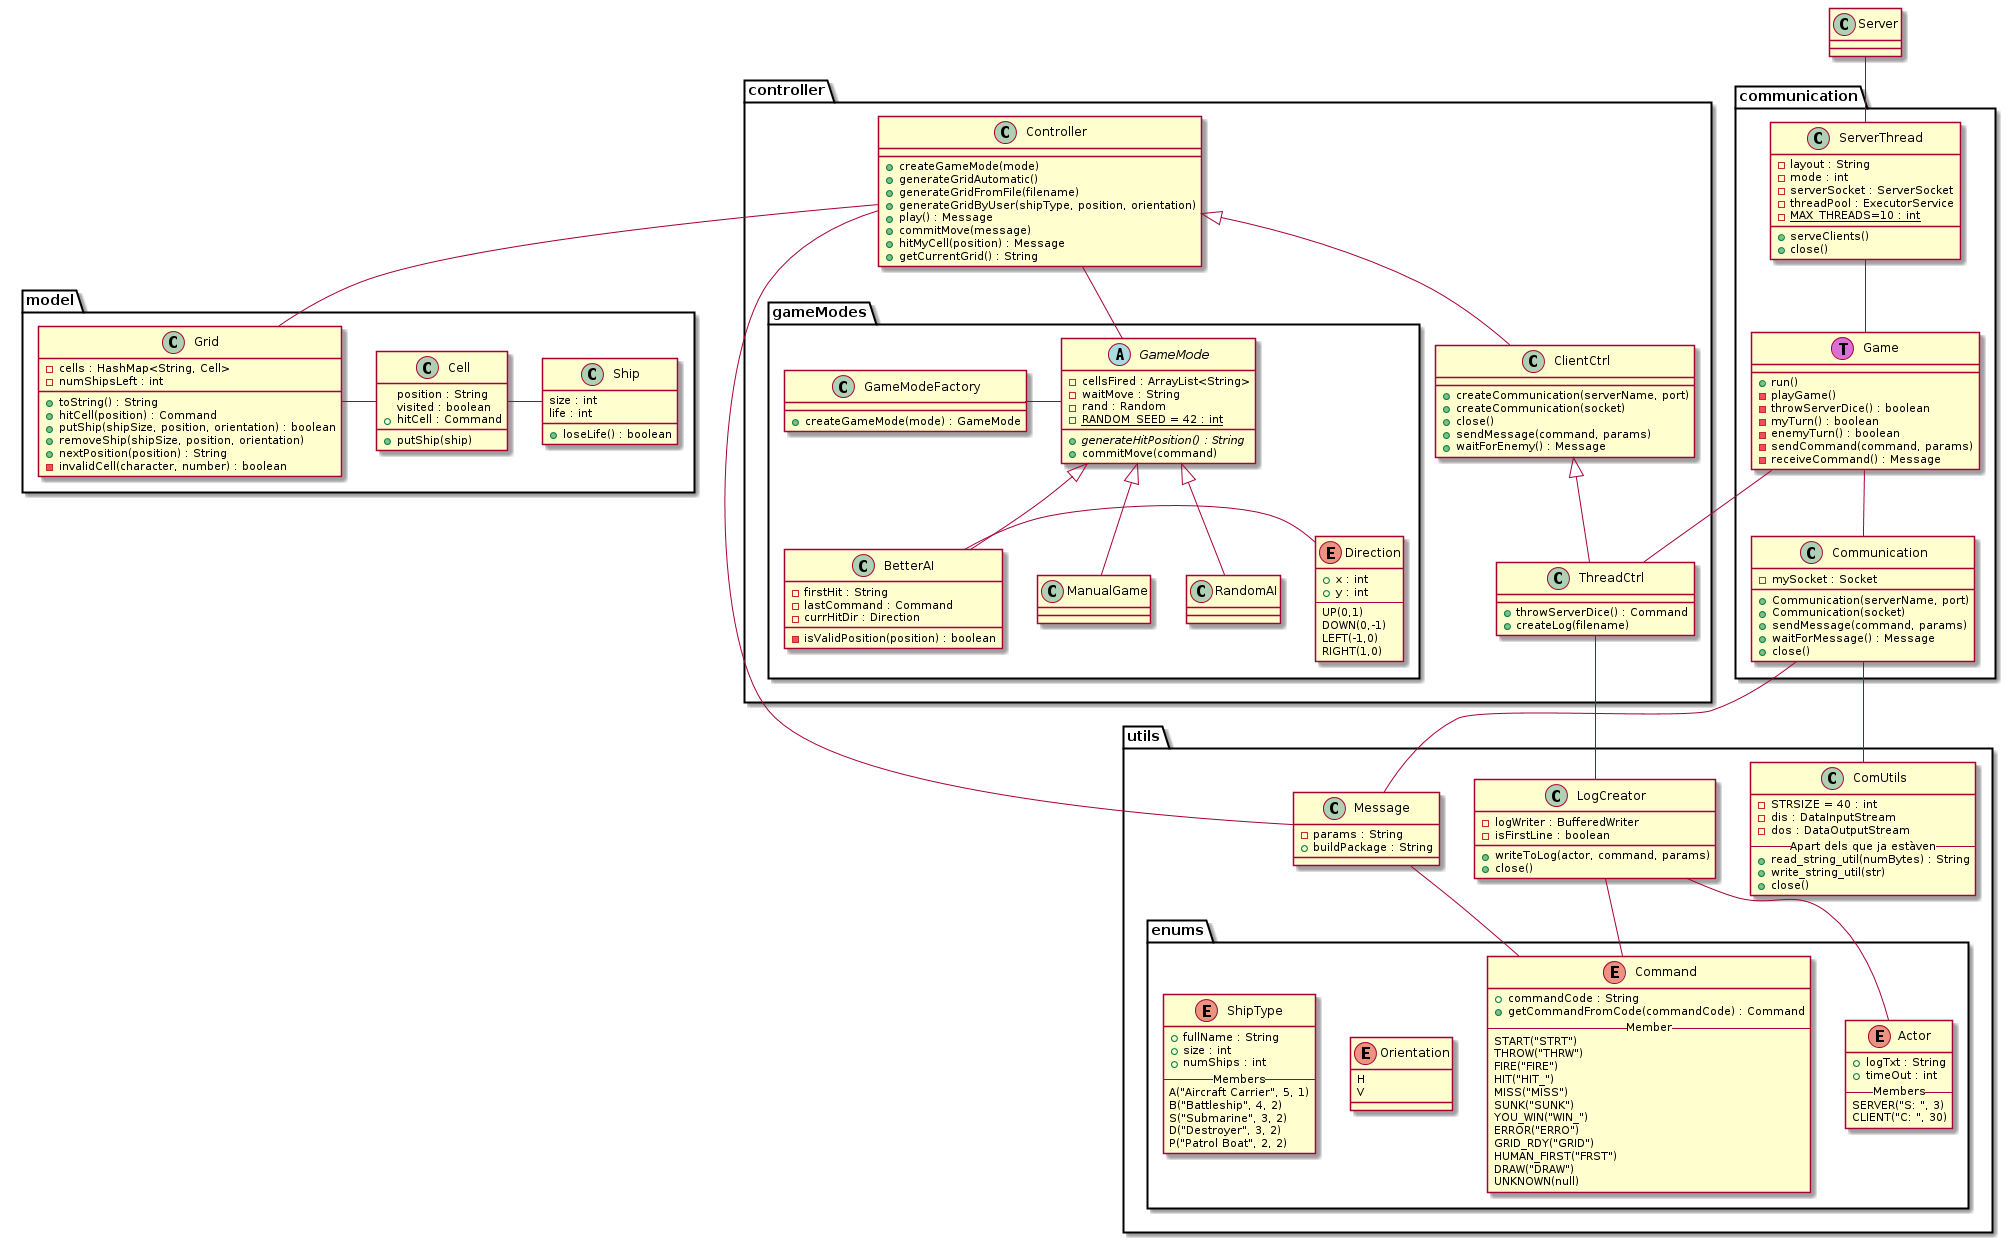
\includegraphics[width=\textwidth,height=\textheight,keepaspectratio]{../diagrams/class-diagrams/threadsClasses.png}
    \caption{Threads-Server Diagram}
    \label{fig:PropProf}
\end{sidewaysfigure}
\begin{sidewaysfigure}[ht]
    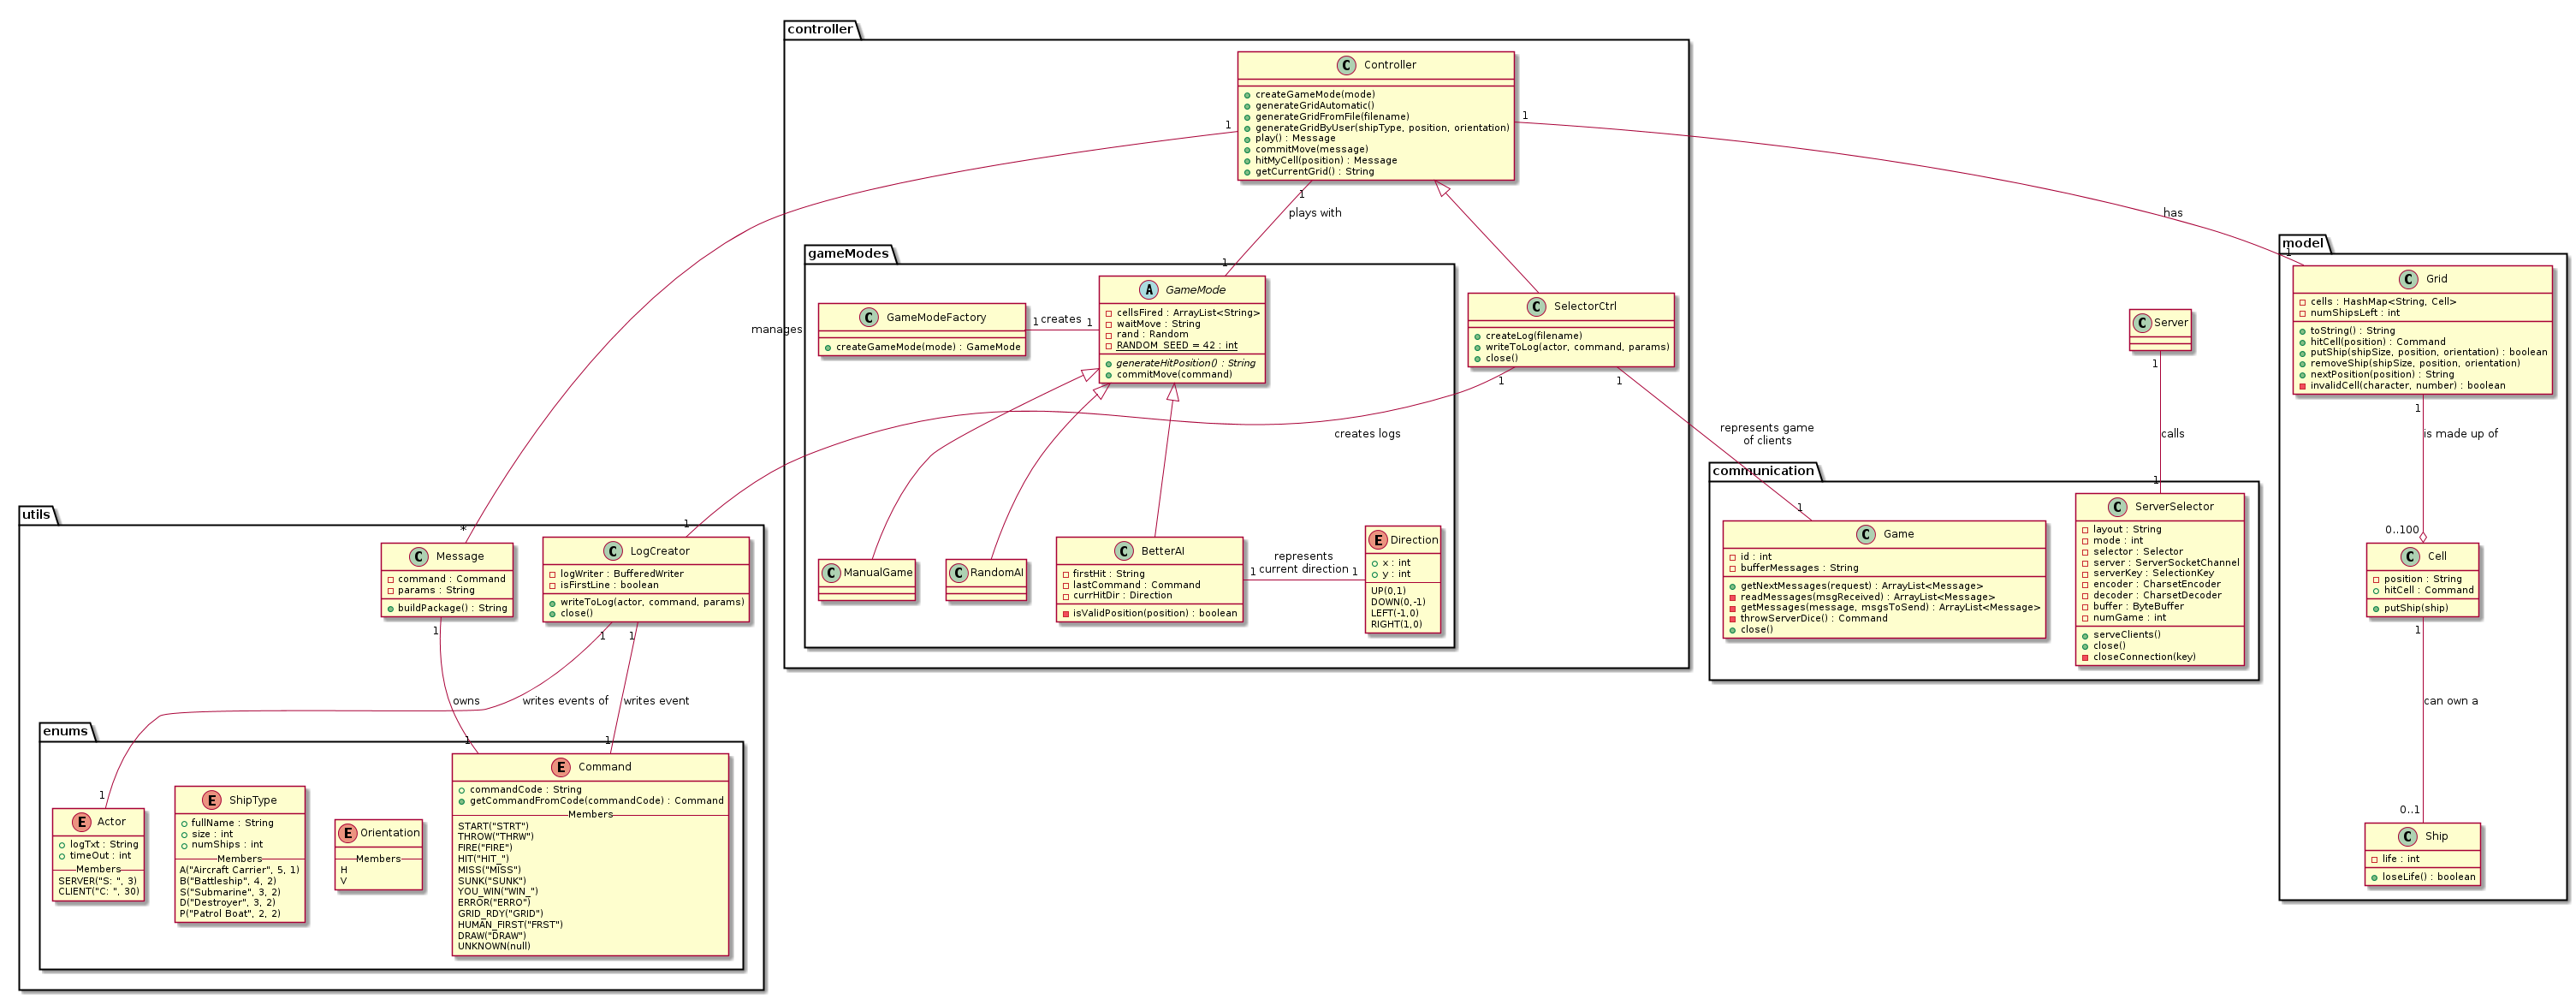
\includegraphics[width=\textwidth,height=\textheight,keepaspectratio]{../diagrams/class-diagrams/selectorClasses.png}
    \caption{Selector-Server Diagram}
    \label{fig:PropProf}
\end{sidewaysfigure}

\end{document}	